\documentclass{mcmthesis}
\mcmsetup{CTeX = false,    % 使用 CTeX 套装时,设置为 true
	tcn = {2504496}, problem = \textcolor{red}{A},
	sheet = true, titleinsheet = true, keywordsinsheet = true,
	titlepage = false, abstract = false}

\usepackage{newtxtext}     % \usepackage{palatino}
\usepackage[style=apa,backend=biber]{biblatex}
\addbibresource{reference.bib}

\usepackage{tocloft}
\setlength{\cftbeforesecskip}{6pt}
\renewcommand{\contentsname}{\hspace*{\fill}\Large\bfseries Contents \hspace*{\fill}}


\title{Enjoy a Cozy and Green Bath}
% \author{\small \href{http://www.latexstudio.net/}
	%   {\includegraphics[width=7cm]{mcmthesis-logo}}}
\date{\today}

\begin{document}

%%%%%%%%%%%%%%%%%%%%%%%%%%%%%%%%%%%%%%%%
%%%%%%%%%%%%%%%%% 摘要 %%%%%%%%%%%%%%%%%
%%%%%%%%%%%%%%%%%%%%%%%%%%%%%%%%%%%%%%%%
\begin{abstract}

abstract...

\begin{keywords}
	Keyword one, Keyword two, Keyword three
\end{keywords}

\end{abstract}


\maketitle
\tableofcontents        % 若不想要目录, 注释掉该句
\thispagestyle{empty}
\newpage





%%%%%%%%%%%%%%%%%%%%%%%%%%%%%%%%%%%%%%%%
%%%%%%%%%%%%%%%%% 引言 %%%%%%%%%%%%%%%%%
%%%%%%%%%%%%%%%%%%%%%%%%%%%%%%%%%%%%%%%%


\section{Introduction}

\subsection{Background}
The medal table of the 2024 Paris Olympics shows that the United States and China each won 40 gold medals and tied for the top spot, but the United States led with a total of 126 medals. The host country France ranked fifth in gold medals (16) and fourth in total medals (64). Dominica, Saint Lucia and other countries won their first Olympic medals, while 60 countries still have not broken through for any medals.
\begin{figure}[htbp]
	\centering
	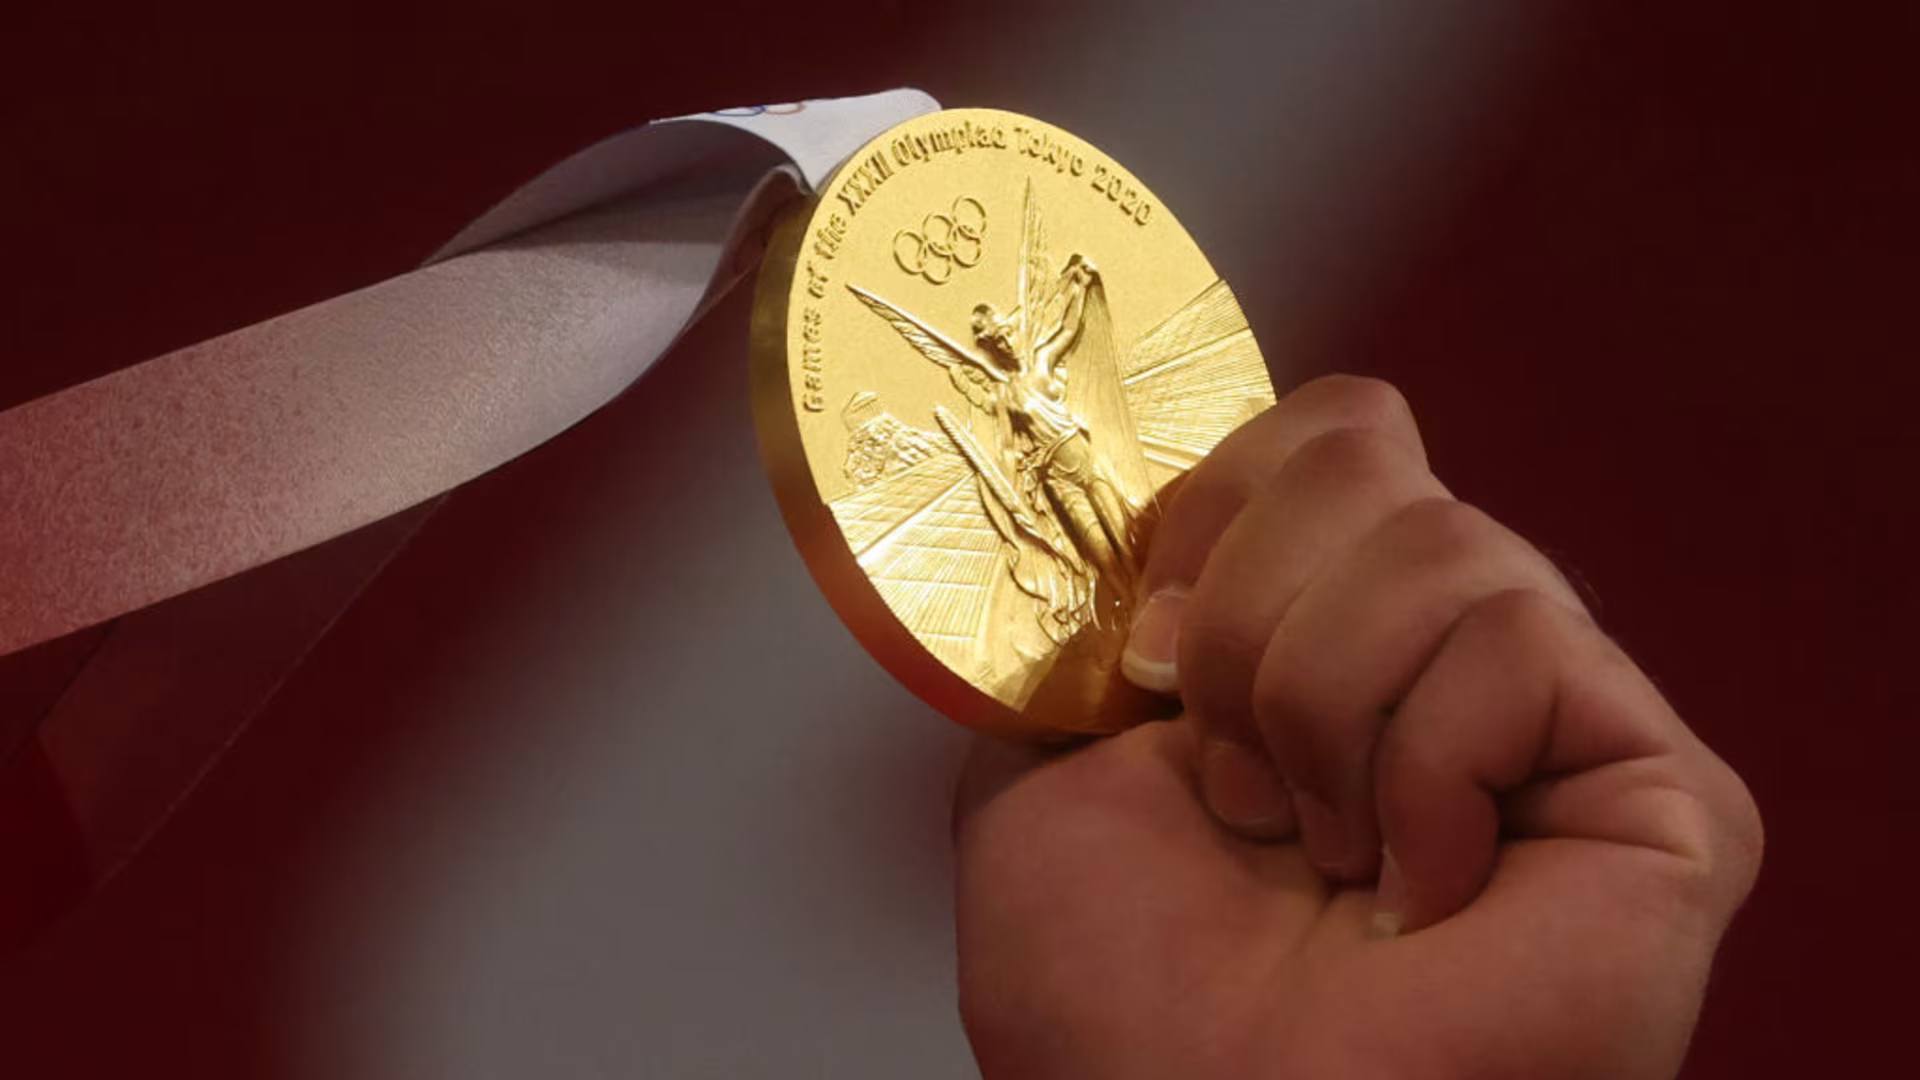
\includegraphics[width=0.7\linewidth]{fig/background}
	\caption{The medals of the 2024 Paris Olympics}
\end{figure}

\subsection{Restatement and Analysis of the Problem}
Based on the provided historical data-set of the Olympic Games from 1896 to 2024, we are employed to analyze and answer the following questions:
\begin{enumerate}
	\item 
	Develop a \textbf{prediction model} to forecast the number of medals each country will win in 2028, and identify countries that may progress or regress. 
	\item 
	Provide \textbf{prediction intervals} and estimates of \textbf{uncertainty} and metrics to measure the model's performance.
	\item 
	Estimate the number of countries that will win their \textbf{first medal} and the probability of this happening.
	\item 
	Analyze the \textbf{relationship} between specific Olympic events (in terms of quantity and type) and the number of medals, explore which events are more important, and the impact of the host country's event selection strategy on the outcome.
	\item 
	Verify whether the \textbf{mobility of coaches} significantly enhances a country's performance in specific sports (such as Lang Ping and Bela Karolyi).
	\item 
	Quantify the contribution of\textbf{ coaching effectiveness} to the number of medals, and recommend key sports for investment and expected returns for the three countries.
	\item 
	Extract the less-attended-to patterns from the model and provide strategic \textbf{suggestions} for the Olympic Committee.
\end{enumerate}

For Task 1, we selected seven indicators and established an LSTM-based medal quantity prediction model, and provided interval predictions using Bayesian estimation. As for countries that have never won medals, we built an SVM-based "first medal breakthrough" prediction model based on the new events, the number of athletes, and historical participation trends.


%对于Task1,我们选取7个指标,建立了基于LSTM的奖牌数量预测模型,并使用贝叶斯估计给出了区间预测,而对于从未获奖的国家,我们根据新增的event、运动员数量、历史参与趋势,建立了基于SVM的“首奖突破”预测模型。
%对于Task2,我们分析了“伟大教练”效应的影响。









\subsection{Overview of Our Work}

%\begin{itemize}
%	\item {\bf 111}. ...
%	\item {\bf 222}. ...
%	
%	\begin{itemize}
%		\item[1)] ... 
%		\item[2)] ...
%		\item[3)] ...
%		\item[4)] ...
%	\end{itemize}
%	
%\end{itemize}








%%%%%%%%%%%%%%%%%%%%%%%%%%%%%%%%%%%%%%%%
%%%%%%%%%%%%%%%%% 模型假设 %%%%%%%%%%%%%%%%%
%%%%%%%%%%%%%%%%%%%%%%%%%%%%%%%%%%%%%%%%
\section{Assumptions and Justification}

To simplify the problem and make it convenient for us to simulate real-life 
conditions, we make the following basic assumptions, each of which is properly 
justified.

\begin{itemize}
	\item {\bf 1}. ...
	\item {\bf 2}. ...	
\end{itemize}










%%%%%%%%%%%%%%%%%%%%%%%%%%%%%%%%%%%%%%%%
%%%%%%%%%%%%%%%%% 符号说明 %%%%%%%%%%%%%%%%%
%%%%%%%%%%%%%%%%%%%%%%%%%%%%%%%%%%%%%%%%
\section{List of Notations}
\begin{center}
\begin{tabular}{ll}
	\toprule
	{\bf Symbols} & {\bf Description}  \\
	\midrule 
	$A_{C},A_{T},A_{S},A_{H}(t)$ & Set of country, years, all sports and host country in year $t$.\\
	$MG_{t,i,j,k}$ & Number of gold medals country $i$ won in sport $j$ at event $k$ in year t. \\
	$MS_{t,i,j,k}$ & Number of silver medals country $i$ won in sport $j$ at event $k$ in year t. \\
	$MB_{t,i,j,k}$ & Number of bronze medals country $i$ won in sport $j$ at event $k$ in year t. \\
	$MT_{t,i}$ & Number of total medals country $i$ won in year $t$. \\
	$N_{athletes}(t,i)$ & Total number of athletes from country $i$ in year $t$. \\
	$N_{award}(t,i)$ & Number of athletes who won medals from country $i$ in year $t$. \\
	$H(t,i)$ & Host effect. \\
	$y_{t,i,j,k}$ &  Logical variable of event $j$ of sport $i$ from $i$ in year $t$. \\
	$G_{\text{growth}}(t,i)$ & Growth rate of the number of athletes from country $i$ in year $t$.\\
	$P_{Medal}(t,i)$ & Probability of country $i$ winning a medal in year $t$ based on the prediction model.\\
	$P_{Gold}(t,i)$ & Based on the prediction model, the probability that country $i$ wins a gold medal in year $t$.\\
	\bottomrule
\end{tabular}
\end{center}

\noindent where we define the main parameters while specific value of those 
parameters will be found in the data-set attached.











%%%%%%%%%%%%%%%%%%%%%%%%%%%%%%%%%%%%%%%%
%%%%%%%%%%%%%%%%% 数据预处理 %%%%%%%%%%%%%%%%%
%%%%%%%%%%%%%%%%%%%%%%%%%%%%%%%%%%%%%%%%
\section{Data Pre-processing}

\subsection{Outlier and Missing Value Handling}
As the \textbf{1906 Intercalated Games} lacked the medal data of various countries and the competition results were not recognized by the International Olympic Committee, the data of 1906 is not taken into account.

In adition, \textbf{Skating} and \textbf{Ice Hockey} have been included in the Winter Olympics since 1920, so these two events are not within the scope of consideration. Otherwise, the "$\cdot$" is replaced by the number $0$. 

It was noticed that \textbf{Jeu de Paume} and \textbf{Roque} sports in the {\bf summerOly\_programs.csv} do not have Codes. Upon researching information from {\color{blue}\url{https://en.wikipedia.org/wiki/Jeu_de_paume}} and {\color{blue}\url{https://en.wikipedia.org/wiki/Roque}}, it was found that only a few people are still engaged in these two sports, which have even not been held for 26 consecutive years in the Summer Olympics. Therefore, these two sports have been excluded.

%\section{Descriptive statistical analysis}


统一国家标识













%%%%%%%%%%%%%%%%%%%%%%%%%%%%%%%%%%%%%%%%
%%%%%%%%%%%%%%%%% Task 1 %%%%%%%%%%%%%%%%%
%%%%%%%%%%%%%%%%%%%%%%%%%%%%%%%%%%%%%%%%
\section{Model 1: Prediction of Number of Medals for Medal-Winning Countries}

\subsection{Significance Analysis of Host Effect}

\textbf{Host Effect} refers to the phenomenon where the host country or region performs more prominently in large-scale international events (such as the Olympic Games, the World Cup, etc.) due to its home field advantage. This phenomenon is usually reflected in a significant increase in the host country's medal count, competition results, or overall performance. 

%为了验证东道主效应的显著性,我们采用了成对样本t检验。首先,我们选取每年的东道主的奖牌数$MT_{ti}$作为第一个样本,其次,为了消除奖牌数量的整体增长趋势的影响,选取东道主国家在前后两届奥运会中获得的奖牌数的平均值

To verify the significance of the host effect, we employed a paired samples \textbf{t-Test}. Firstly, we selected the medal count of the host country in each year, denoted as $MT_{t}$, as the first sample. Secondly, to eliminate the influence of the overall growth trend in medal counts, we took the average of the medal counts obtained by the host country in the two consecutive Olympic Games as the second sample, shown as (\ref{eq:H_t-test_MT_bar}),
\begin{equation}
MT^H_{t}=\frac{ MT_{t-1} + MT_{t+1} }{2}
\label{eq:H_t-test_MT_bar}
\end{equation}
where $t\in A_T^H = A_T \textbackslash \{1896,2024\}$, $i\in A_{C}$. 

Then $\{MT_{t},MT^s_{t}\}$ constitutes paired data with a sample size of 30. Define $d_t= MT_{t} - MT^s_{t}$, and assume that
\begin{equation*}
H_0: \mu_d=0, \quad vs \quad H_1:  \mu_d \ne 0.
\end{equation*}

Select the t-test statistic as
\begin{equation}
t=\frac{ \bar{d} }{ s_d\slash \sqrt{30} } \sim T(29)
\end{equation}
where $\bar{d}=\frac{1}{30} \sum_{t\in A_T^H} d_t$ is the mean of paired samples, 
and $ s_d = \frac{1}{29} \sum_{t\in A_T^H}\big( d_t - \bar{d} \big)^2 $ is the sample variance of the differences of paired data, 

For a given significance level $\alpha$, the rejection domain for the hypothesis test is
\begin{equation}
W_\alpha = \big\{ |t| \ge T_{1-\frac{\alpha}{2}}(29) \big\}
\end{equation}

By following the described procedure, the results of the t-test were obtained and are summarized in Table \ref{table:H_t-test_result}.

结果待写



\subsection{Index Analysis}
为了
\subsubsection{Host effect}

Define Logical Variable $H_{t,i}$ as equation (\ref{eq:H}),
\begin{equation}
	H_{t,i}=
	\begin{cases}
		1, \quad \text{Country } i \text{ is host in year } t, \\
		0, \quad \text{others}.
	\end{cases}
	\label{eq:H}
\end{equation}
where $t\in A_{T}$, $i\in A_{C}$.



\subsubsection{Events}
The event vector \( V(t) \) is defined as:

\[
V(t) = \big( v_1(t), v_2(t), \dots, v_M(t) \big)^T,
\]
where: \( v_i(t) = 1 \) if event \( i \) is held in year \( t \),
\( v_i(t) = 0 \) if event \( i \) is not held in year \( t \). Here, \( M \) represents the total number of distinct Olympic events considered up to year \( t \), and the elements of \( V(t) \) are binary values indicating the participation of each event in year \( t \).

\subsubsection{Formal Definition}

For any event \( i \) and year \( t \), we define \( v_i(t) \) as follows:

\[
v_i(t) =
\begin{cases}
	1 & \text{if event } i \text{ is held in year } t, \\
	0 & \text{if event } i \text{ is not held in year } t.
\end{cases}
\]


\subsubsection{Definition of Dominant Event}

Let \( I_j(t) \) represent the dominance of event \( j \) in year \( t \), where the dominance is calculated based on the medal count over the past three years and the total number of medals in year \( t \).
\[
I_j(t) = \frac{\sum_{q=t-3}^{t-1} MT_{q,i,k,j}}{\sum_{q=t-3}^{t-1}V_j(q) \cdot MT{q,i,j,k}} 
\]
where the formula calculates the dominant position of country $i$ in year  $t$  for event  $j$ , determined by the ratio of past medal performance to the total number of medals in that year, adjusted for the presence of the event in the last three years.







\subsubsection{Other indexes}




\subsection{LSTM Model}







\section{Model 2: Prediction of Maiden Medal for Medal-Less Countries}


\subsection{Problem Overview}
The objective of this model is to predict whether countries that have never won a medal in the past (i.e., "first-time winning countries") will be able to win a medal in future Olympic Games. For these countries, traditional medal prediction models (which usually rely on historical medal data) may not effectively predict their future performance. Therefore, we need to consider other potential factors, such as the host country effect, athlete participation growth, and the addition of new events.


\subsection{Index Analysis}


\subsubsection{Target variable}
\[
y(t,i) = 
\begin{cases} 
	1 & \text{if country } i \text{ wins a medal in year } t \\ 
	0 & \text{if country } i \text{ does not win a medal in year } t 
\end{cases}
\]
\subsubsection{Athlete growth rate}
The growth rate of athletes from country $i$ in year $t$, calculated by the following formula:
\[
G_{\text{growth}}(t,i) = \frac{N_{\text{participate}}(t,i) - N_{\text{participate}}(t-1,i)}{N_{\text{participate}}(t-1,i)}
\]
where $N_{\text{participate}}(t,i)$ is the number of athletes from country $i$ in year $t$.


\subsubsection{Participation in new events compared to previous years} 
\[
N_{\text{new}}(t,i) =
\begin{cases}
	1 & \text{if } N_{\text{new}}(k,i) > 0, \quad k = t-8\ or\ t-4\ or\ t \\
	0 & \text{if } N_{\text{new}}(k,i) = 0, \quad k = t-8, t-4, t
\end{cases}
\]

where $N_{\text{new}}(t,i)$ represents the number of new events that country $i$ participated in during year $t$. The term $\Delta N_{\text{new}}(t,i)$ indicates the change in the number of new events from the past three years to year $t$.





\textbf{Prediction model}:
We use a Support Vector Machine (SVM) model to predict whether first-time winning countries will win medals. The model’s input is the feature vector of the country $X(t,i)$:
\[
X(t,i) = [G_{\text{growth}}(t,i), H(t,i), N_{\text{new}}(t,i)]
\]
By training the SVM model, we can obtain the probability that country $i$ will win a medal in year $t$:
\[
P(\text{Medal}(t,i)) = f(X(t,i), \theta)
\]
where $f(\cdot)$ is the decision function learned through SVM, and $\theta$ is the parameter learned during training.

\textbf{Prediction of first-time medal probability}:
If country $i$ has never won a medal (i.e., no historical medals), we use the prediction model to calculate the probability of winning a medal. If the probability exceeds a certain threshold, we predict that the country may win a medal in the future, especially a first-time medal:
\[
P_{\text{first medal}}(t,i) = P(\text{Medal}(t,i)) > \text{Threshold}
\]
where the threshold is determined based on the results of model evaluation.






















\section{Task 2: xxx}

\section{Task 3: xxx}

\section{Task 4: xxx}

\section{Sensitivity Analysis}

\section{Strength and Weakness}
\subsection{Strength}
\subsection{Weakness}

\section{Further Discussion}



%%%%%%%%%%%%%%%%%%%%%%%%%%%%%%%%%%%%%%%%
%%%%%%%%%%%%%%%%% Memo信 %%%%%%%%%%%%%%%%%
%%%%%%%%%%%%%%%%%%%%%%%%%%%%%%%%%%%%%%%%
\newpage
\section*{Memo} % 无编号标题
\addcontentsline{toc}{section}{Memorandum} % 手动添加到目录

\begin{letter}{Enjoy Your Bath Time!}


\vspace{\parskip}

Sincerely yours,

Your friends

\end{letter}










%%%%%%%%%%%%%%%%%%%%%%%%%%%%%%%%%%%%%%%%
%%%%%%%%%%%%%%%%% 文献条目 %%%%%%%%%%%%%%%%%
%%%%%%%%%%%%%%%%%%%%%%%%%%%%%%%%%%%%%%%%
\newpage
\section*{Reference} % 无编号标题
\addcontentsline{toc}{section}{References} % 手动添加到目录
\printbibliography




%%%%%%%%%%%%%%%%%%%%%%%%%%%%%%%%%%%%%%%%
%%%%%%%%%%%%%%%%% 附录 %%%%%%%%%%%%%%%%%
%%%%%%%%%%%%%%%%%%%%%%%%%%%%%%%%%%%%%%%%
\begin{appendices}
\section{First appendix}
\section{Second appendix}
\end{appendices}




%%%%%%%%%%%%%%%%%%%%%%%%%%%%%%%%%%%%%%%%
%%%%%%%%%%%%%%%%% AI使用 %%%%%%%%%%%%%%%%%
%%%%%%%%%%%%%%%%%%%%%%%%%%%%%%%%%%%%%%%%
\newpage
\newcounter{lastpage}
\setcounter{lastpage}{\value{page}}
\thispagestyle{empty} 

\section*{Report on Use of AI}

\begin{enumerate}
\item OpenAI ChatGPT (Nov 5, 2023 version, ChatGPT-4,) 
\begin{description}
	\item[Query1:] <insert the exact wording you input into the AI tool> 
	\item[Output:] <insert the complete output from the AI tool>
\end{description}
	
\item OpenAI ChatGPT (Nov 5, 2023 version, ChatGPT-4,) 
\begin{description}
	\item[Query1:] <insert the exact wording you input into the AI tool> 
	\item[Output:] <insert the complete output from the AI tool>
\end{description}

\end{enumerate}

% 重置页码
\clearpage
\setcounter{page}{\value{lastpage}}






\end{document}